\documentclass[12pt]{article}
\usepackage{light}
\usepackage{verbatim}
%\hidesolutions
\showsolutions

%%%%% some macros needed %%%%%%%%%%%
\newcommand{\eqdef}{\mathbin{::=}}
\newcommand{\mfigure}[3]{\bigskip\centerline{\resizebox{#1}{#2}{\includegraphics{#3}}}\bigskip}
\newcommand{\edge}[2]{#1\text{---}#2}
\newcommand{\arc}[2]{#1\!\longrightarrow\!#2}
\newcommand{\beqn}{\begin{eqnarray*}}
\newcommand{\eeqn}{\end{eqnarray*}}
\newcommand{\ok}{\marginpar{ok?}}
%%%%%%%%%%%%%%%%%%%%%%%%%%%%%%%%%%%%%

\begin{document}

\recitation{7}{October 1, 2014}
\section{Build-up error}
Recall a graph is \term{connected} iff there is a path between every pair of its vertices.

\begin{falseclm*}
If every vertex in a graph has positive degree, then the graph is
connected.
\end{falseclm*}

\begin{enumerate}[(a)]

\item Prove that this Claim is indeed false by providing a
counterexample.

\solution{
There are many counterexamples; here is one:

\begin{figure}[!h]
\centering
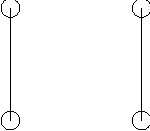
\includegraphics[scale = 0.75]{false-connect-cx}
\end{figure}
}

\item Since the Claim is false, there must be a logical mistake in the
following bogus proof.  Pinpoint the \emph{first} logical mistake
(unjustified step) in the proof.

\begin{proof}
  We prove the Claim above by induction.  Let $P(n)$ be the proposition
  that if every vertex in an $n$-vertex graph has positive degree, then
  the graph is connected.

\textbf{Base cases}: ($n \leq 2$).  In a graph with 1 vertex, that vertex
cannot have positive degree, so $P(1)$ holds vacuously.

$P(2)$ holds because there is only one graph with two vertices of positive
degree, namely, the graph with an edge between the vertices, and this
graph is connected.

\textbf{Inductive step}: We must show that $P(n)$ implies
$P(n+1)$ for all $n \geq 2$.  Consider an $n$-vertex graph in which every
vertex has positive degree.  By the assumption $P(n)$, this graph is
connected; that is, there is a path between every pair of vertices.  Now
we add one more vertex $x$ to obtain an $(n+1)$-vertex graph:

\mfigure{!}{1.75in}{false-connect-pic}

All that remains is to check that there is a path from $x$ to every other
vertex $z$.  Since $x$ has positive degree, there is an edge from $x$ to
some other vertex, $y$.  Thus, we can obtain a path from $x$ to $z$
by going from $x$ to $y$ and then following the path from $y$ to $z$.  This
proves $P(n+1)$.

By the principle of induction, $P(n)$ is true for all $n \geq 0$, which
proves the Claim.

\end{proof}

\solution{
This one is tricky: the proof is actually a good proof of
something else.  The first error in the proof is only in the final
statement of the inductive step: ``This proves $P(n+1)$''.

What we have actually shown (above) is that there are graphs on n+1 vertices
where each vertex has positive degree, and are connected. But if we want to
show that every graph on n+1 vertices where each vertex has positive
degree, is
necessarily connected, when we start with G and try to remove a node and all
edges incident to it we do not necessarily get a graph on n vertices that
satisfies the conditions we want. To put it more succinctly, in the
counterexample to part (a) every vertex we choose to delete results in a graph
where some node has degree zero afterwards.

\noindent \textit{Inductive step:} We must show that $P(n)$ implies
$P(n+1)$ for all $n \geq 1$.  Consider an $(n+1)$-vertex graph $G$ in
which every vertex has degree at least 1.  Remove an arbitrary vertex
$v$, leaving an $n$-vertex graph $G'$ in which every vertex has
degree... uh-oh!

The reduced graph $G'$ might contain a vertex of degree 0, making the
inductive hypothesis $P(n)$ inapplicable!  We are stuck--- and
properly so, since the claim is false!
}

\end{enumerate}

\section{Euler tours}

\emph{The statement of (a) in the original version was incorrect! This has been corrected below.}

\begin{enumerate}[(a)]
    \item Prove that a graph $G$ has an Euler tour if and only if every vertex of $G$ has even degree.

Note that there are two directions to prove!

\solution{
    The proof is the same as in the proof of Theorem 5.6.3 in the book (pp.~159--160).
}
\item Suppose that $G$ is strongly connected. (A strongly connected graph is one in which any vertex can be reached from any other). Come up with a necessary and sufficient condition for the existence of an Euler tour in a \emph{directed} graph. Adapt your proof above to prove that your condition is the right one.
    %Adapt your proof above to show that in a directed graph, an Eulerian circuit exists if and only if for every vertex, the indegree equals the outdegree.
%\emph{(Once you've figured out the condition, you might want to skip writing down the proof until you've done the rest of the recitation.)}

    \solution{The condition is: an Euler tour exists if and only if for every vertex, the indegree equals the outdegree.

        The proof is basically the same. 
        Any Euler tour must enter and exit a vertex the same number of times; so the condition is certainly necessary. 
        
        Now suppose the condition holds, and let $W = w_0, w_1, \ldots, w_k$ be a longest walk in $G$ using every directed edge at most once. 
        Then $W$ must be a closed walk; for suppose that $w_k \neq w_0$. Then we must have entered $w_k$ one more time than we left it, which means that there is some outgoing directed edge that we have not used. This would allow us to extend the walk, contradicting that $W$ was as long as possible.

        Suppose that $W$ is not an Euler tour. 
        Either $W$ contains all vertices or it does not. First consider the case that all vertices are
        in $W$. Because it is not an Euler tour, there is at least one edge not used. Given this edge,
        there must be an unused edge out of the end of this edge. If there weren't, that would contradict
        the assumption that the indegree equals the outdegree and $W$ is a closed walk. We can continue to
        follow this chain of edges. The only thing that can stop this is getting to the start of the
        first edge since this would allow the chain to stop. This chain is a closed walk all not in $W$.
        We can combine the closed walks which makes a longer walk, contradicting the assumption that
        $W$ was the longest.

        Now, suppose that not all vertices are in $W$. There must be an unused edge directed away from some vertex in the walk $W$; for if not, there would be no path from any vertex on $W$ to a vertex not in $W$, contradicting the assumption that $G$ is strongly connected.  
        Let $w_i \to u$ be this edge. Construct a walk $W'$ beginning with this edge and traversing only unused edges, stopping when we cannot make a move. Again by the condition that indegree equals outdegree, this walk will end at $w_i$. We thus obtain a longer walk 
        \[ W' = w_0, w_1, \ldots, w_i, u, \ldots, w_i, w_{i+1}, \ldots, w_k. \]
        This is again a contradiction.

    }

    \begin{comment}
\item Based on your proof of b), give an algorithm to find an Euler tour, when one exists, in the directed case. % Your algorithm should be reasonably efficient.

    \solution{
        
        \begin{enumerate}
            \item Let $W = v_0$, where $v_0$ be an arbitrary vertex. Let $E' = E$.
            \item Repeat until $E'$ is empty
                \begin{enumerate}
                    \item Choose any vertex $v_i$ in the walk $W$ that is adjacent to some edge in $E'$
                    \item Do a walk $W' = v_i, w_1, w_2, \ldots, w_k$ in $G'=(V, E')$ that starts at $v_i$ and that uses each edge at most once, until no steps are possible. This walk will end at $w_k = v_i$.
                        Remove all edges of this walk from $E'$.
                        Replace $W = v_0, v_1, \ldots, v_i, \ldots, v_k$ with the walk
                        \[ v_0, \ldots, v_i, w_1, \ldots, w_{k-1}, v_i, \ldots, v_k. \]
                \end{enumerate}
        \end{enumerate}
    } 
\end{comment}
%
%        Choose an arbitrary vertex $v_0$, and begin walking from this node, at each step choosing an arbitrary outgoing directed edge. 
%        Once an edge is traversed, remove it from the graph (burn your bridges so to speak).
%        Eventually, this walk gets stuck; say we get the walk $v_0, v_1, \ldots, v_k$. 
%        Since we're stuck, and indegree is equal to outdegree at all vertices, it must be that $v_k = v_0$. So we have a closed walk.
%
%        
%        If there are any remaining edges, we will extend our walk.
%        Let $W = v_0, v_1, \ldots, v_k=v_0$ be the closed walk we have so far, and let $v_i$ be any node which touches some remaining edges. 
%        (Note that if we have used every edge that touches a node in the walk, we must have used all edges, since the graph is connected.)
%        Then do a walk $v_i, w_1, w_2, \ldots, w_r$ of unused edges starting from $v_i$. Again, this must stop at $v_i$. We can thus splice this together with $W$ to obtain a longer closed walk
%        \[ v_0, v_1, \ldots, v_i, w_1, w_2, \ldots, w_{r-1}, v_i, v_{i+1}, \ldots, v_k. \]
%        We continue this process, each time getting a longer walk, until we've exhausted all the edges. 
%    }

\end{enumerate}

\section{Connectivity}

Prove that any simple graph with $n$ nodes and strictly more than $\tfrac12(n-1)(n-2)$ edges is connected.
%\emph{(Hint: try to prove the equivalent statement that any disconnected graph on $n$ nodes has at most $(n-1)(n-2)/2$ edges.}
\solution{
    We'll show the equivalent statement that any disconnected graph on $n$ nodes has at most $(n-1)(n-2)/2$ edges.

    Let $G=(V,E)$ be any graph on $n$ nodes that is not connected. Then there must be more than one connected component; let $G_1 = (V_1, E_1)$ be any connected component, and let $G_2 = (V_2, E_2)$ be the graph induced on $V_2 := V - V_1$. 
    Note that there are no edges going between $G_1$ and $G_2$, and so $E_1 \cup E_2 = E$.

    How many edges can $G_1$ have? At most ${|V_1| \choose 2}$ edges (one for each pair of nodes). Similarly, $G_2$ can have at most ${|V_2| \choose 2}$ edges. 

    Write $t := |V_1|$; then $|V_2| = |V| - |V_1| = n - t$.
    So the total number of edges in $G$ is at most
    \[ \frac{t(t-1)}{2} + \frac{(n-t)(n-t-1)}{2}. \]
    If we simplify this, we get
    \[ |E| \leq \frac{n(n-1)}{2} - t(n-t). \]
    But since $1 \leq t \leq n-1$, $t(n-t) \geq n-1$. (You can confirm this with some calculus; it might help to draw $t(n-t)$ as a function of $t$; it's just a parabola.) So 
    \[ |E| \leq \frac{n(n-1)}{2} - (n-1) = \frac{(n-2)(n-1)}{2}. \]
}
\end{document}
